\begingroup
\setlength{\textfloatsep}{0.7em}
\setlength{\floatsep}{0.7em}
\setlength{\abovecaptionskip}{0.35ex}
\setlength{\belowcaptionskip}{0.2em}

\newcommand{\vfplaceholderfigure}[5]{%
\begin{figure}[htbp]
\centering
\IfFileExists{images/#1}{%
\includegraphics[width=#2\linewidth,height=#3\textheight,keepaspectratio]{images/#1}%
}{%
\fbox{%
\begin{minipage}[c][#3\textheight][c]{#2\textwidth}
\centering
VietFlood figure placeholder\\[0.3cm]
Suggested content: #4\\[0.25cm]
File name:\\[0.1cm]
\resizebox{0.9\linewidth}{!}{\texttt{#1}}
\end{minipage}%
}%
}%
\caption{#4}
\label{#5}
\end{figure}%
}

This chapter discusses the execution of the VietFlood prototype, as well as the concrete deliverables produced by the project. The system was put in place to offer a complete reporting loop: users authenticate, citizens submit a report with location and optional proof, the backend stores and serves that report via a stable API, and administrators examine and update report status.

The implementation comprises four main artifacts: 1) a backend consisting of an API gateway, an authentication service and a reports service; 2) a mobile application for citizen and relief users; 3) a web dashboard for administrators; and 4) a shared library, \texttt{vietflood\_common} providing reusable infrastructure across services.

\section{Prototype Deliverables and Tech Stack}

For consistency in models, validation rules, and data contracts while development, TypeScript is used in both the server and the client apps. The backend services are developed using NestJS \cite{nestjsDocs} and the NestJS microservice support is used to interact over a message broker \cite{nestjsMicroservicesDocs}. The mobile application is constructed using Expo React Native \cite{expoDocs,reactNativeDocs} and the web dashboard is built using Next.js \cite{nextjsDocs}.

The prototype is designed to run in containers. For local development, Docker Compose is used to launch the gateway, services, RabbitMQ, and Redis in a repeatable environment \cite{dockerComposeDocs}. For deployment, container images are deployed to Azure App Service \cite{azureAppServiceContainersDocs} and build/deploy automation is done with GitHub Actions \cite{githubActionsDocs}. Sensitive parameters such as the database URL, JWT secrets, Cloudinary credentials, and broker credentials are passed in using environment variables and not saved in source code.

\begin{table}[htbp]
\centering
\caption{Technologies employed in the VietFlood prototype.}
\label{tab:vietflood-implementation-tools}
\setlength{\tabcolsep}{8pt}
\renewcommand{\arraystretch}{1.18}
\footnotesize
\begin{tabular}{|p{3.2cm}|p{9.3cm}|}
\hline
\textbf{Component} & \textbf{Implementation choices} \\
\hline
Backend & NestJS services, TypeORM persistence, RabbitMQ communication, Redis cache, and JWT authentication. \\
\hline
Shared library & \texttt{vietflood\_common} for logging, Redis helpers, and Cloudinary upload utilities. \\
\hline
Evidence storage & Cloudinary for media uploads and public delivery URLs. \\
\hline
Mobile app & Expo React Native, secure token storage, image picker, and location services. \\
\hline
Web dashboard & Next.js, role-based routes, report review UI, and admin status updates. \\
\hline
Deployment & Docker Compose for local runtime, GitHub Actions automation, and containers on Azure App Service. \\
\hline
\end{tabular}
\end{table}

\section{Implementation of the Backend}

\subsection{Responsibilities for Routing and Service}

API gateways are the sole components of the infrastructure that are accessible to clients. It handles HTTP requests, including multipart uploads, verifies access using guards, and dispatches internal work to the authentication or reporting service. Internal communication uses RabbitMQ request--response message patterns \cite{rabbitmqConfirmsDocs,nestjsMicroservicesDocs}. It keeps transport and access control together, and moves business logic and database operations into separate services.

\begin{table}[htbp]
\centering
\caption{Distribution of responsibility among backend services in VietFlood.}
\label{tab:service-roles-vietflood}
\footnotesize
\setlength{\tabcolsep}{5pt}
\renewcommand{\arraystretch}{1.2}
\begin{tabular}{|p{3.0cm}|p{9.4cm}|}
\hline
\textbf{Service} & \textbf{Main responsibilities} \\
\hline
API gateway & Public REST routes, file parsing for uploads, JWT and role guards, and routing requests to internal services. \\
\hline
Auth service & User registration, password validation, token issuance, refresh token rotation, and user administration. \\
\hline
Reports service & Report persistence, evidence metadata storage, report listing and filtering, status updates, and cache invalidation. \\
\hline
\end{tabular}
\end{table}

\vfplaceholderfigure
{figure4-1-rabbitmq-communication-flow.png}
{0.74}
{0.28}
{Message routing from the API gateway to internal services through RabbitMQ.}
{fig:vietflood-rabbitmq-flow}

\FloatBarrier
\subsection{Authentication, Tokens and Role Checks}

VietFlood employs password authentication. We hash passwords with bcrypt before storage \cite{provos1999bcrypt}. After login the authentication service returns an access token and refresh token. Access tokens are JSON Web Tokens that hold identity and role claims needed by the gateway authorization guards \cite{jones2015jwt}. Refresh tokens are saved and rotated to enable longer-lived sessions and to reduce the impact of a token leak.

The prototype has three supported roles: \texttt{citizen}, \texttt{relief} and \texttt{admin}. Protected endpoints and admin-only routes have role checks at gateway. This is a simplistic model, but it is sufficient to illustrate the distinct responsibilities: residents submit reports, relief users browse and watch, and administrators assess and alter status.

\begin{figure}[htbp]
\centering
\begin{minipage}[t]{0.31\linewidth}
\centering
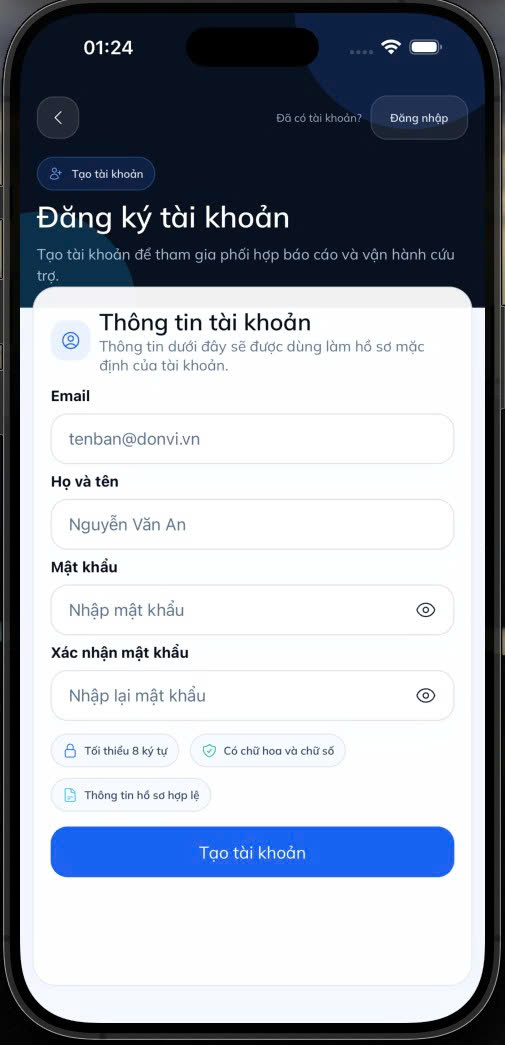
\includegraphics[width=0.88\linewidth,height=0.27\textheight,keepaspectratio]{images/figure4-2-mobile-registration.jpg}\\
\small Citizen registration view.
\end{minipage}
\hfill
\begin{minipage}[t]{0.31\textwidth}
\centering
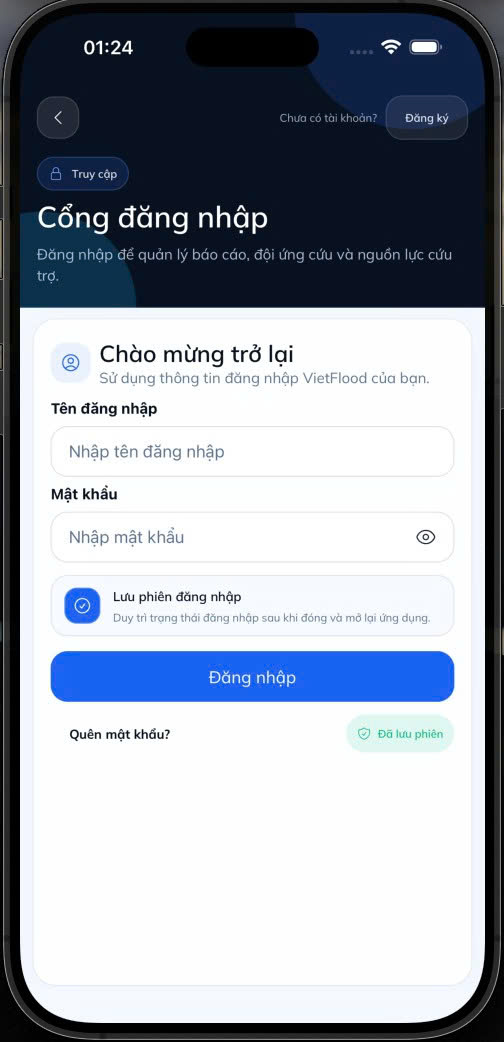
\includegraphics[height=0.27\textheight,width=0.88\linewidth,keepaspectratio]{images/figure4-3-mobile-login.jpg}\\
\small Mobile sign-in view.
\end{minipage}
\hfill
\begin{minipage}[t]{0.31\textwidth}
\centering
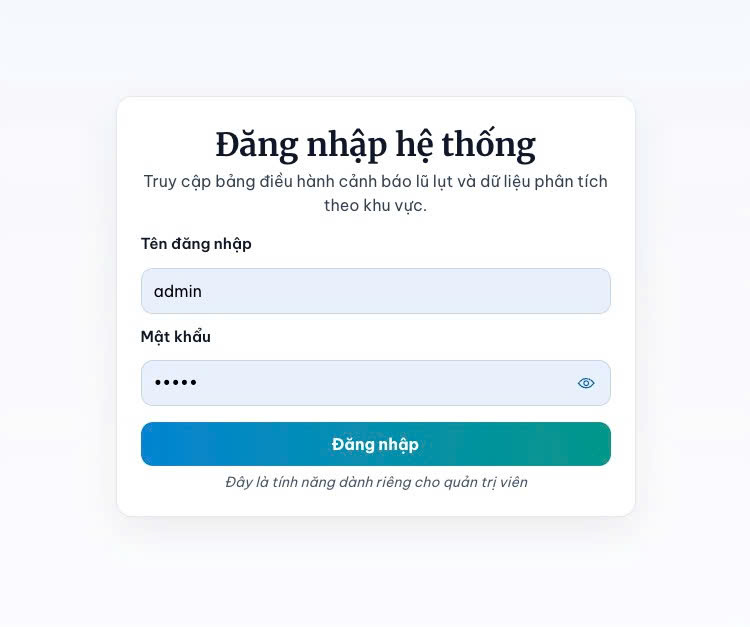
\includegraphics[width=\linewidth,height=0.27\textheight,keepaspectratio]{images/figure4-4-web-admin-login.jpg}\\
\small Administrator sign-in view.
\end{minipage}
\caption{Authentication screens for citizen registration, mobile login, and administrator login.}
\label{fig:vietflood-auth-screens}
\end{figure}

\vfplaceholderfigure
{figure4-6-token-refresh-flow.png}
{0.74}
{0.26}
{Refresh token rotation sequence to get new access tokens and invalidate old refresh tokens.}
{fig:vietflood-refresh-token-flow}

\FloatBarrier
\subsection{Evidence Pipeline and Report Handling}

Flood reports are produced from the mobile client and received by the gateway as multipart form data. In the presence of evidence photos, the gateway uploads files to Cloudinary and creates a list of metadata, including delivery URL, public ID, and resource type \cite{cloudinaryUploadDocs}. The final payload is subsequently transmitted to the reports service via RabbitMQ. The reports service validates the payload, persists the report using TypeORM \cite{typeormDocs}, and writes a cache item in Redis for speedier subsequent lookups \cite{redisDocs}.

This evidence-first pipeline keeps the database focused on structured report fields but still makes evidence available for evaluation. It also makes the report contents self-contained; administrators can review a report by reading one database row plus associated evidence information, without requiring local file storage.

\vfplaceholderfigure
{figure4-7-report-processing-flow.png}
{0.74}
{0.26}
{End-to-end report processing pipeline from submission to persistence and cache refresh.}
{fig:vietflood-report-processing-flow}

Update and remove actions are subject to the same service boundary. The gateway enforces role permissions and passes update/delete orders to the reports service. The reports service invalidates and updates cache entries when a report changes so that subsequent reads match the current state.

\FloatBarrier
\subsection{Utilities for Shared Infrastructure}

In order to keep services minimal and consistent, VietFlood contains a shared library, \texttt{vietflood\_common}, exposing a logging module and modest wrappers for Redis and Cloudinary. Centralization of these utilities minimizes duplicated code and facilitates consistent error handling and configuration across services.

\vfplaceholderfigure
{figure4-8-common-library-structure.png}
{0.72}
{0.25}
{Shared utility package used by backend services for logging, Redis, and Cloudinary.}
{fig:vietflood-common-lib}

\FloatBarrier
\subsection{Live Location Event Channel}

The prototype uses a Socket.IO gateway for live location broadcasting \cite{socketioDocs}. Clients submit \texttt{send-location} events with lat and long values. The gateway checks the coordinate ranges and publishes valid updates to other connected clients using a \texttt{receive-location} event. Invalid payloads cause a \texttt{location-error} response to the sender. This feature displays event flow as it occurs. It can be enhanced with authorized identities and persistence if needed for operational use.

\vfplaceholderfigure
{figure4-9-live-tracking-flow.png}
{0.72}
{0.25}
{Socket.IO location event flow including validation, broadcast, and error response.}
{fig:vietflood-flow-live-tracking}

\FloatBarrier
\section{Client Side Implementation}

\subsection{Mobile App Capabilities}

The mobile application provides the field-facing interface, and is designed for rapid submission and reading. Once signed in the app loads the current profile and shows a report list for the user. Citizens can fill in a category, a short description, administrative address fields and coordinates and generate a report. The make report request includes the selection and upload of evidence photographs from the device.

The relief role is related to map and browsing views. Relief users can view report listings and inspect report details, although they do not modify report status in this prototype. That separation prevents competing status updates and keeps the verification decision inside the administrator workflow.

\begin{figure}[htbp]
\centering
\begin{minipage}[t]{0.31\linewidth}
\centering
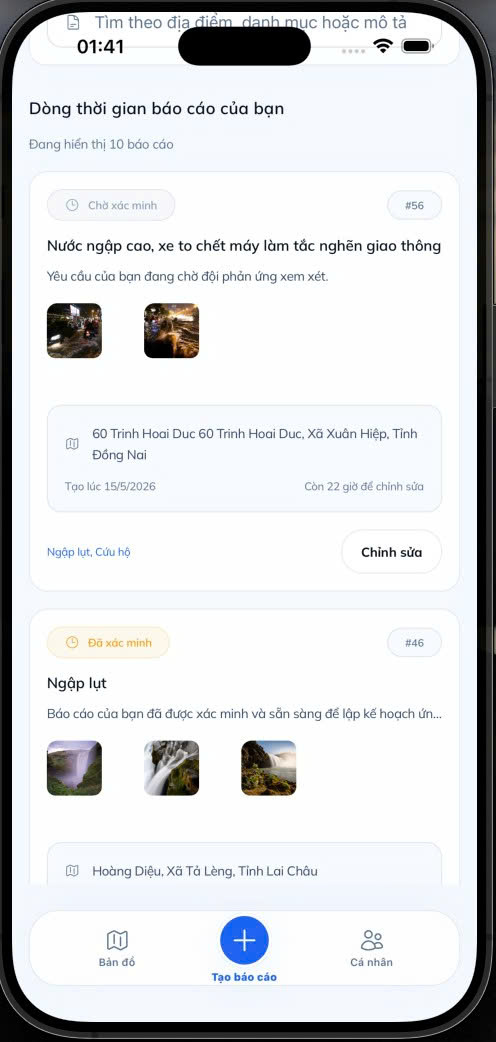
\includegraphics[width=0.88\linewidth,height=0.27\textheight,keepaspectratio]{images/figure4-10-mobile-report-list.jpg}\\
\small Citizen report list.
\end{minipage}
\hfill
\begin{minipage}[t]{0.31\textwidth}
\centering
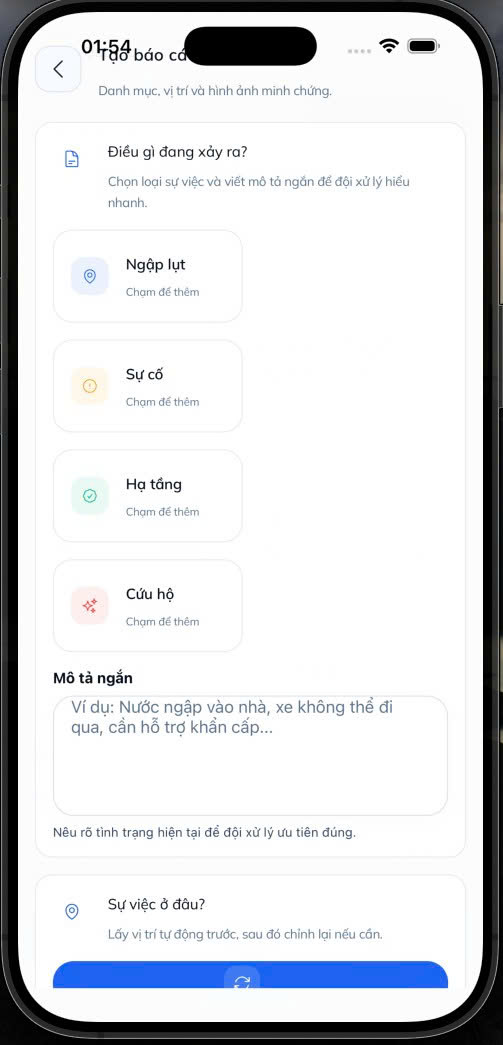
\includegraphics[width=0.88\linewidth,height=0.27\textheight,keepaspectratio]{images/figure4-11-mobile-create-report.jpg}\\
\small Report creation form.
\end{minipage}
\hfill
\begin{minipage}[t]{0.31\textwidth}
\centering
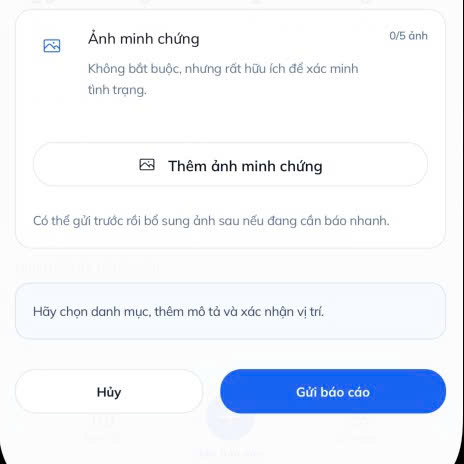
\includegraphics[width=0.88\linewidth,height=0.27\textheight,keepaspectratio]{images/figure4-12-mobile-evidence-upload.jpg}\\
\small Evidence upload workflow.
\end{minipage}
\caption{Mobile application screens for report listing, report creation, and evidence upload.}
\label{fig:vietflood-mobile-report-flow}
\end{figure}

\begin{figure}[htbp]
\centering
\begin{minipage}[t]{0.44\linewidth}
\centering
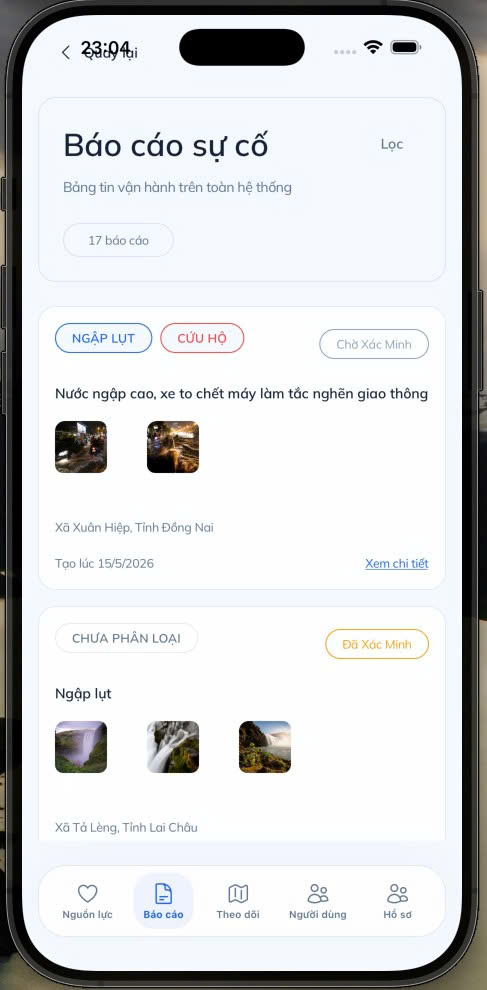
\includegraphics[width=0.72\linewidth,height=0.28\textheight,keepaspectratio]{images/figure4-13-relief-report-list.jpg}\\
\small Relief list view.
\end{minipage}
\hfill
\begin{minipage}[t]{0.44\linewidth}
\centering
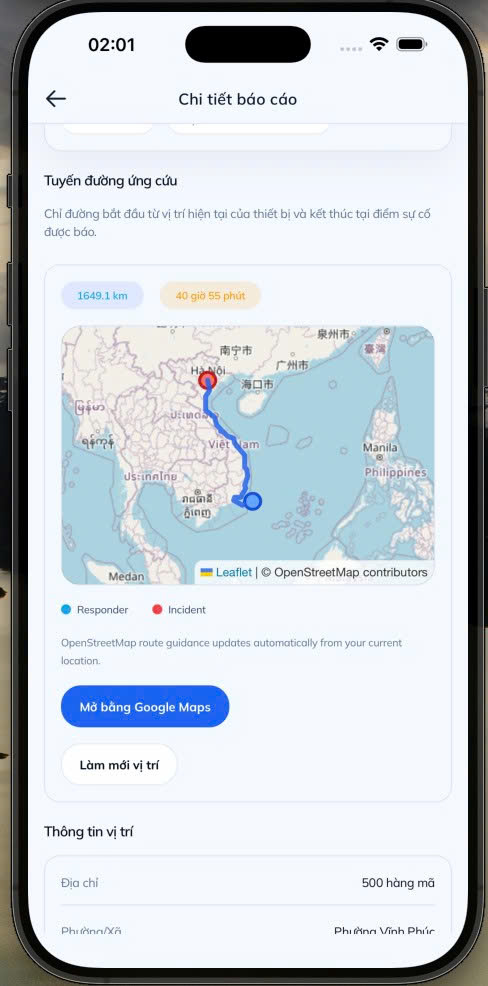
\includegraphics[width=0.72\linewidth,height=0.28\textheight,keepaspectratio]{images/figure4-14-relief-map.jpg}\\
\small Relief map view.
\end{minipage}
\caption{Relief user screens for browsing reports and viewing their spatial distribution.}
\label{fig:vietflood-relief-screens}
\end{figure}

\FloatBarrier
\subsection{Admin Panel Features}

The online dashboard handles report review and user administration. This loads the current profile after login and prevents routes that require admin access. Administrators can view incoming reports, filter them by status, see evidence thumbnails and change status values such as \texttt{pending}, \texttt{verified}, \texttt{resolved} and \texttt{rejected}. Status changes are delivered to the gateway and then sent to the reports service over RabbitMQ to keep the database and cache coherent.

\vfplaceholderfigure
{figure4-15-admin-dashboard-overview.jpg}
{0.82}
{0.27}
{Administrator dashboard overview showing report cards, filters, and evidence thumbnails.}
{fig:vietflood-admin-dashboard-summary}

\vfplaceholderfigure
{figure4-16-admin-evidence-status-update.jpg}
{0.82}
{0.29}
{Evidence review and status update screen for administrators.}
{fig:vietflood-admin-evidence-status}

\clearpage
\section{Automating Release and Deployment}

The prototype runtime is containerized for consistency between local and deployed environment. For local development, Docker Compose is utilized to launch all dependencies, Redis and RabbitMQ, in addition to the backend services \cite{dockerComposeDocs}. Images are created and published, and Azure App Service is set up to execute the most recent images using environment configuration supplied by the platform \cite{azureAppServiceContainersDocs}. This is a straightforward container-based deployment method.

Automation is done with GitHub Actions to produce images, submit them to a registry and update the deployment configuration \cite{githubActionsDocs}. In line with continuous delivery approach, which maintains build and deploy logic in version-controlled pipelines \cite{humble2010continuousDelivery,kim2016devopsHandbook}, this minimizes manual processes.

\vfplaceholderfigure
{figure4-17-cicd-workflow.png}
{0.80}
{0.26}
{CI/CD pipeline from source push to container build, publish and Azure App Service deployment.}
{fig:vietflood-cicd-workflow}

\FloatBarrier
\section{Summary of the Results}

VietFlood can be launched locally with Docker Compose and exercised via the mobile and web clients at the final stage of implementation. The backend exposes REST endpoints for authentication and report administration via the API gateway. A complete list of endpoints is described in Appendix~A, Table~\ref{tab:appendix-api-endpoints}, with representative response samples utilized in the evaluation.

In practice, the system exhibits the expected function split: residents submit reports, relief users explore location-aware views and administrators analyze and amend report status. These results are assessed in Chapter~5 using scenario walkthroughs and functional test checklists.

\vfplaceholderfigure
{figure4-18-user-management.jpg}
{0.80}
{0.28}
{User management view to browse accounts and responsibilities in the dashboard.}
{fig:vietflood-usermanagement}

\FloatBarrier
\endgroup
